\documentclass[11pt,a4paper]{report}
\usepackage[utf8]{inputenc}
\usepackage[french]{babel}
\usepackage[T1]{fontenc}
\usepackage{amsmath}
\usepackage{amsfonts}
\usepackage{amssymb}
\usepackage{xcolor}
\usepackage{gensymb}

\usepackage{geometry}
\geometry{hmargin=2.5cm,vmargin=1.5cm}
\usepackage{wasysym}
\usepackage{graphicx}

\author{Mathieu Sarrat}
\title{LC1 - Chimie et Couleur}

\makeatletter
\renewcommand{\thesection}{\@arabic\c@section}
\makeatother


\begin{document}
\maketitle

\section*{Niveau, Pré-requis et objectifs}

\subsubsection*{Niveau}
\begin{itemize}
	\item \textbf{Niveau :} Terminale STL, SPCL\\
\end{itemize}

\subsubsection*{Matériel}
\begin{itemize}
	\item \textbf{Synthèse et caractérisation de l'aspirine : voir le Maréchal};
	\item \textbf{Extraction de l'anéthole : voir plus bas};
	\item Matériel de CCM (plaques, échantillons, tubes capillaires, pots de confiture et solvants pour 		les éluants, lampe UV pour révélation;
\end{itemize}

\subsubsection*{Instructions}
\begin{itemize}
	\item En préparation, faire la synthèse de l'aspirine et la filtration pour avoir le solide brut 		impur :
		\begin{itemize}
			\item garder une fraction de produit impur pour le premier point de fusion et la CCM;
			\item recristalliser le reste en préparation, ne faire que la filtration en direct;
			\item 
		\end{itemize}
Prélever la moitié du solide pour la recristallisation/filtration. Laisser sécher l'autre moitié à l'étuve. 
\end{itemize}

\newpage
\section*{Introduction}

Après une synthèse, plusieurs produits peuvent être formés. Il peut aussi rester des réactifs si la réaction n'est pas totale. Il y a également le solvant. Cet ensemble est appelé "brut réactionnel". \`A partir du brut, il est alors nécessaire de séparer les différentes espèces, de les purifier au mieux, et enfin de contrôler la pureté du produit fini. Les techniques utilisées varient, notamment en fonction de la nature des produits.\\

Nous allons présenter et mettre en œuvre plusieurs techniques expérimentales de séparation, de purification et de contrôle de pureté dans le cas où le produit à récupérer est soit un solide, soit un liquide.

\section{L'aspirine}\label{sec:1}

\textcolor{blue}{Voir Le Maréchal tome 2 et la leçon molécules de la santé pour le protocole détaillé.}
Obtenir en préparation le brut réactionnel (après filtration, on ne conserve que le produit solide).

\subsection{Analyse du brut réactionnel}

\begin{itemize}
	\item Présenter la réaction réalisée, les espèces chimiques et les quantités utilisées.\\
	
	\item On peut caractériser la pureté d'un solide en mesurant son point de fusion. Si le solide 			n'est pas pur (i.e. c'est un mélange), la température de fusion est plus faible que celle du 			composé pur. \textcolor{blue}{Manip :} Présenter le banc Köfler. On étalonne avec un composé ayant 		une température de fusion entre 130\degree C et 140\degree C. . Mesurer le point de fusion et 			constater la présence d'impuretés. Ne pas oublier de nettoyer le banc (nettoyer avec un coton 			imbibé d'éthanol de la zone chaude à la zone froide).
\end{itemize}

\subsubsection*{Données :}
\begin{itemize}
	\item Point de fusion de l'acide acétylsalicylique : 138\degree C.
	\item Point de fusion de l'acide salicylique : 158\degree C.
\end{itemize}

\subsection{Purification par recristallisation}

\textcolor{blue}{Voir le Maréchal et leçon Molécules de la Santé pour les détails. Conserver une petite partie du brut réactionnel pour la CCM.}

\textcolor{blue}{Expliquer le principe :} la recristallisation est une technique de base pour purifier les solides. Elle repose sur la différence de solubilité entre le composé à purifier et ses impuretés dans le solvant choisi. Par hypothèse, nous supposerons que les impuretés sont en quantité bien plus faible que le produit à purifier. La solubilité d'un composé augmente généralement avec la température. Ainsi, on dissout le composé à purifier dans le minimum de solvant nécessaire pour le dissoudre, porté à ébullition. Par refroidissement, la solution se sature en composé à purifier (l'excédent précipite, c'est lui qu'on veut récupérer) mais les impuretés restent dissoutes.\\

L'idéal est d'avoir un produit insoluble à froid, soluble à chaud et des impuretés plus solubles à chaud et à froid. On met juste la quantité de solvant nécessaire pour dissoudre à chaud le solide, de sorte qu'il puisse cristalliser quasi-totalement à froid. Le processus de recristallisation étant lent, les impuretés ne sont pas piégées dans le solide et peuvent être éliminées.

\subsection{Séparation liquide/solide}

On doit maintenant éliminer la phase liquide (le solvant) utilisée pour la recristallisation.

\textcolor{blue}{Manip : filtration sur Buchner}. Expliquer le principe de la trompe à eau et de la filtration sous vide. Réaliser la manip en direct. Triturer le solide, laver à l'eau froide.

\subsection{Contrôle de pureté}

Nous avons purifié l'acide acétylsalicylique. Contrôlons son degré de pureté.

\subsubsection*{Chromatographie sur couche mince ou spectro IR}

\textcolor{blue}{Voir le Maréchal pour la composition de l'éluant. On peut aussi ne pas la faire et la réserver au cas de l'anéthol, et parler de spectroscopie IR à la place (voir leçon Molécules de la Santé pour les spectres)}\\

\textcolor{blue}{Expliquer le principe :} on joue sur les différences d'affinité (polarité) entre les échantillons, la silice de la phase fixe et le solvant de la phase mobile. Ces différences se traduisent par une migration plus ou moins prononcée des échantillons le long de la plaque une fois que celle-ci a été trempée dans l'éluant (mélange de solvants dont le choix et les proportions dépendent des échantillons à analyser). 

Faire quatre dépôts :
\begin{itemize}
	\item 1 produit non recristallisé;
	\item 2 produit recristallisé;
	\item 3 acide acétylsalicylique pur;
	\item 4 acide salicylique pur;\\
\end{itemize}

Pendant que les espèces migrent, faire le point de fusion (paragraphe suivant).\\

Révélation à l'UV.

Déterminer le rapport frontal :
\begin{equation}
	R_f = \frac{h}{H}
\end{equation}
où h désigne la hauteur atteinte par la tache et H la hauteur atteinte par le front de l'éluant.

\subsubsection*{Point de fusion}

\begin{itemize}
	\item \textcolor{blue}{Refaire une mesure de point de fusion sur le banc Köfler, en repartant de 			l'endroit où le brut réactionnel a fondu.} Conclure.\\ 
\end{itemize}

\subsubsection*{Rendement (probablement pas faisable)}

Faire un calcul de rendement en pesant le produit pur :
	\begin{equation}
		\eta = \frac{\xi_f}{\xi_{max}} = \frac{m_\text{produit}}{M_\text{produit}}\times
		\frac{M_\text{réactif}}{m_\text{réactif}}.
	\end{equation}

\newpage
\section{L'anéthole}\label{sec:2}

L'anéthole est présent dans la badiane, le fenouil, et surtout dans l'anis. On l'utilise comme matière première dans la fabrication de liqueurs, et en médecine comme stimulant et aromatisant.

\subsection{Décoction}

La décoction est une méthode très ancienne, qui consiste à placer la substance que l'on souhaite extraire dans de l'eau froide, que l'on porte ensuite à ébullition pour en dissoudre les constituants.

\subsubsection*{Matériel nécessaire}
\begin{itemize}
	\item erlenmeyer de 100 mL;
	\item bécher de 150 mL;
	\item réfrigérant à air;
	\item barreau aimanté et agitateur magnétique chauffant;
	\item élévateur pour montage à reflux;
	\item filtre papier plissé, entonnoir de verre, tubes à essais;
	\item ampoule à décanter;
	\item matériel de CCM (révélation aux UV);
	\item réfractomètre.
\end{itemize}

\subsubsection*{Produits nécessaires}
\begin{itemize}
	\item 4 g d'anis étoilé broyé (décoction);
	\item cyclohexane, chlorure de sodium solide (extraction);
	\item sulfate de magnésium anhydre (séchage);
	\item dichlorométhane (CCM);
	\item anéthole dilué à 2\% dans le cyclohexane (CCM);\\
\end{itemize}

\textbf{Remarque :} on peut aussi procéder par macération, comme proposé sur le Mesplède-Randon : on introduit l'anis étoilé en poudre dans du dichlorométhane (manipuler impérativement sous la hotte), à froid, et on met sous vive agitation pendant trente à quarante minutes. On ajoute de l'eau pour chasser l'eau de la phase organique, dans une ampoule à décanter. Le dichlorométhane étant plus dense que l'eau, la phase organique sera au bas de l'ampoule.

\begin{figure}[h!]
	\begin{center}
		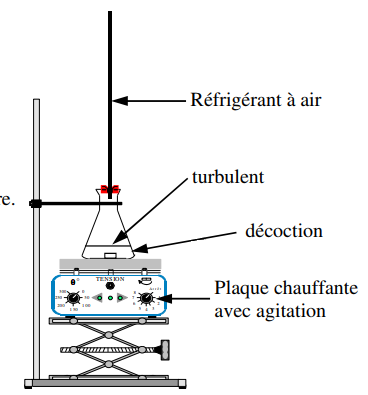
\includegraphics[scale=0.5]{montage_reflux.png}
	\end{center}
\end{figure}

\subsubsection*{Protocole}
\begin{itemize}
	\item Introduire l'anis étoilé broyé dans l'erlenmeyer;
	\item Ajouter 20 à 30 mL d'eau chaude;
	\item Adapter le réfrigérant à air selon le schéma ci-contre;
	\item Chauffer à reflux 15 minutes environ, puis laisser refroidir;
	\item Filtrer afin de recueillir le filtrat.
\end{itemize}

Utilité du réfrigérant à air : on recondense les vapeurs, pour ne pas perdre de l'anéthole.

\subsection{Extraction liquide-liquide}

\begin{itemize}
	\item Verser le filtrat dans l'ampoule à décanter;
	\item Dissoudre 3 g de chlorure de sodium;
	\item Extraire avec 2 fois 3 mL de cyclohexane;
	\item Recueillir dans un tube à essais à la phase organique.
\end{itemize}

\subsubsection*{Principe de l'ampoule à décanter}

On joue sur la différence de solubilité entre le solvant contenant le produit à extraire et le solvant utilisé pour l'extraction. Ces deux solvants doivent être peu miscibles entre eux. On introduit d'abord le filtrat (solution aqueuse), puis le solvant d'extraction (le cyclohexane). On agite vigoureusement en dégazant de temps en temps, pour évacuer l'excédent de pression. On laisse décanter.\\

La phase la plus dense se trouve au bas de l'ampoule. 

\subsubsection*{Ajout de chlorure de sodium}

L'ajout de chlorure de sodium permet deux choses :
\begin{itemize}
	\item l'anéthole est insoluble dans l'eau salée : on favorise son passage dans le cyclohexane;
	\item l'ajout de chlorure de sodium permet de densifier la phase aqueuse.
\end{itemize}

\subsubsection*{Extractions multiples}

Il vaut mieux faire deux extractions avec un volume V/2 de solvant plutôt qu'une seule extraction avec un volume V : on extrait davantage de produit (meilleur rendement).

\subsection{Séchage}

Il faut ensuite sécher la phase organique, pour éliminer les dernières traces d'eau. On utilise pour cela du sulfate de magnésium anhydre, un solide.

\subsubsection*{Protocole}
\begin{itemize}
	\item Introduire une pointe de spatule de sulfate de magnésium anhydre dans le tube à essais;
	\item Boucher. Agiter vigoureusement une bonne minute durant;
	\item Bien maintenir le bouchon, une petite surpression étant susceptible de se produire;
	\item Si la solution reste trouble, ou si le sulfate de magnésium semble "mouillé", 
	rajouter une nouvelle fois un peu de sulfate et agiter à nouveau. 
\end{itemize}

\subsection{Filtration}

On doit maintenant éliminer le sulfate de magnésium : on procède par filtration, en utilisant un entonnoir et du papier filtre plissé.

\subsection{Contrôle de pureté}

\subsubsection*{Chromatographie}

On procède par CCM.
La plaque est préparée avec 2 dépôts :
\begin{itemize}
	\item un premier dépôt avec le filtrat,
	\item le second avec l'huile essentielle d'anéthole du commerce diluée 
	à 2\% dans le cyclohexane (2 gouttes dans 5 mL).
\end{itemize}

L'éluant utilisé pour le développement est le dichlorométhane (3 à 4 mL). Révéler aux UV.\\
 
Déterminer le rapport frontal :
\begin{equation}
	R_f = \frac{h}{H}
\end{equation}
où h désigne la hauteur atteinte par la tache et H la hauteur atteinte par le front de l'éluant. 

\subsubsection*{Réfractométrie}

\textcolor{blue}{On mesure l'indice de réfraction (l'indice de l'anéthole va de 1.5590 à 1.5620)}. Cette mesure nous permet d'identifier la nature du produit et de contrôler sa pureté.\\

https://www.fishersci.fr/shop/products/trans-anethole-99-acros-organics-3/10149931\\

http://culturesciences.chimie.ens.fr/content/le-refractometre-916

\section*{Conclusion}

On aurait pu parler d'un grand nombre d'autres techniques d'extraction, utilisées par exemple en parfumerie :
\begin{itemize}
	\item \textbf{l'hydrodistillation} consiste à chauffer un mélange d'eau et de substances 					organiques. Le mélange se vaporise et s'enrichit en composés les moins volatils (on ne peut pas 		toujours atteindre une composition de 100\%, s'il y a un azéotrope). Ces vapeurs sont 					recondensées dans un réfrigérant puis récupérées pour la suite du traitement. Le liquide 				récupéré, appelé distillat, est constitué de deux phases : \textbf{l'huile essentielle} (la 			phase organique) qui contient la majorité des composés odorants (car ils sont de nature 				organique) et \textbf{l'eau aromatique} (la phase aqueuse, ), qui en contient peu;\\
	\item \textbf{l'entraînement à la vapeur} repose sur un principe similaire à ceci près que le 				produit organique n'est pas chauffé directement : on envoie de la vapeur d'eau à son contact;\\
	\item \textbf{l'enfleurage}, reposant sur le pouvoir d'absorption d'une huile essentielle par les 			corps gras (à chaud ou à froid). Ce procédé permet de traiter les fleurs fragiles dont l'odeur 			ne survit pas à une élévation de la température. Le processus dure plusieurs mois.\\
	\item la macération (ou la décoction), selon le protocole choisi pour l'anéthole.
\end{itemize}

\end{document}